% Created by tikzDevice version 0.12.6 on 2024-06-15 18:35:17
% !TEX encoding = UTF-8 Unicode
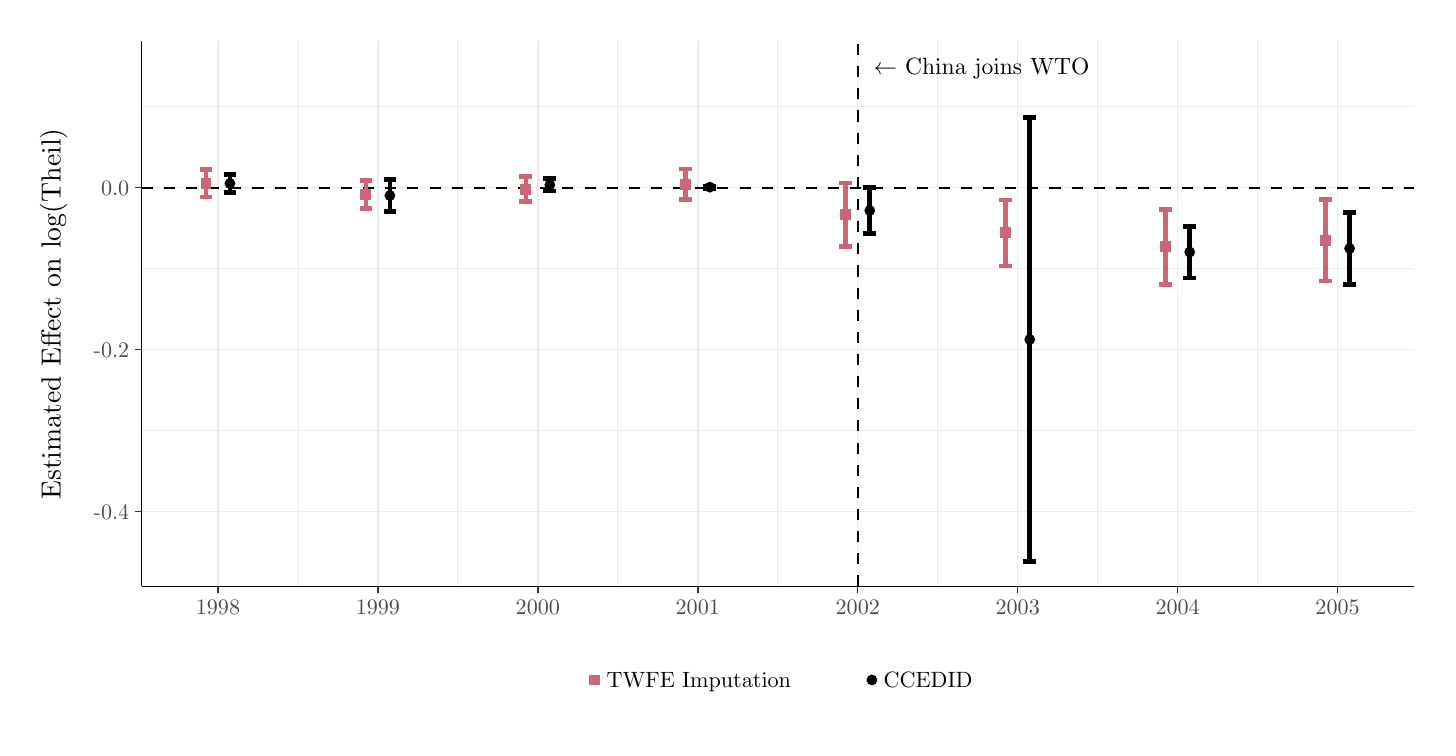
\begin{tikzpicture}[x=1pt,y=1pt]
\definecolor{fillColor}{RGB}{255,255,255}
\path[use as bounding box,fill=fillColor] (0,0) rectangle (505.89,252.94);
\begin{scope}
\path[clip] (  0.00,  0.00) rectangle (505.89,252.94);
\definecolor{drawColor}{RGB}{255,255,255}

\path[draw=drawColor,line width= 0.5pt,line join=round,line cap=round,fill=fillColor] (  0.00, -0.00) rectangle (505.89,252.94);
\end{scope}
\begin{scope}
\path[clip] ( 41.22, 51.02) rectangle (500.89,247.95);
\definecolor{fillColor}{RGB}{255,255,255}

\path[fill=fillColor] ( 41.22, 51.02) rectangle (500.89,247.95);
\definecolor{drawColor}{gray}{0.92}

\path[draw=drawColor,line width= 0.3pt,line join=round] ( 41.22,107.27) --
	(500.89,107.27);

\path[draw=drawColor,line width= 0.3pt,line join=round] ( 41.22,165.82) --
	(500.89,165.82);

\path[draw=drawColor,line width= 0.3pt,line join=round] ( 41.22,224.36) --
	(500.89,224.36);

\path[draw=drawColor,line width= 0.3pt,line join=round] ( 97.66, 51.02) --
	( 97.66,247.95);

\path[draw=drawColor,line width= 0.3pt,line join=round] (155.46, 51.02) --
	(155.46,247.95);

\path[draw=drawColor,line width= 0.3pt,line join=round] (213.25, 51.02) --
	(213.25,247.95);

\path[draw=drawColor,line width= 0.3pt,line join=round] (271.05, 51.02) --
	(271.05,247.95);

\path[draw=drawColor,line width= 0.3pt,line join=round] (328.85, 51.02) --
	(328.85,247.95);

\path[draw=drawColor,line width= 0.3pt,line join=round] (386.65, 51.02) --
	(386.65,247.95);

\path[draw=drawColor,line width= 0.3pt,line join=round] (444.45, 51.02) --
	(444.45,247.95);

\path[draw=drawColor,line width= 0.5pt,line join=round] ( 41.22, 78.00) --
	(500.89, 78.00);

\path[draw=drawColor,line width= 0.5pt,line join=round] ( 41.22,136.54) --
	(500.89,136.54);

\path[draw=drawColor,line width= 0.5pt,line join=round] ( 41.22,195.09) --
	(500.89,195.09);

\path[draw=drawColor,line width= 0.5pt,line join=round] ( 68.76, 51.02) --
	( 68.76,247.95);

\path[draw=drawColor,line width= 0.5pt,line join=round] (126.56, 51.02) --
	(126.56,247.95);

\path[draw=drawColor,line width= 0.5pt,line join=round] (184.36, 51.02) --
	(184.36,247.95);

\path[draw=drawColor,line width= 0.5pt,line join=round] (242.15, 51.02) --
	(242.15,247.95);

\path[draw=drawColor,line width= 0.5pt,line join=round] (299.95, 51.02) --
	(299.95,247.95);

\path[draw=drawColor,line width= 0.5pt,line join=round] (357.75, 51.02) --
	(357.75,247.95);

\path[draw=drawColor,line width= 0.5pt,line join=round] (415.55, 51.02) --
	(415.55,247.95);

\path[draw=drawColor,line width= 0.5pt,line join=round] (473.35, 51.02) --
	(473.35,247.95);
\definecolor{drawColor}{RGB}{0,0,0}

\path[draw=drawColor,line width= 0.6pt,dash pattern=on 4pt off 4pt ,line join=round] ( 41.22,195.09) -- (500.89,195.09);

\path[draw=drawColor,line width= 0.6pt,dash pattern=on 4pt off 4pt ,line join=round] (299.95, 51.02) -- (299.95,247.95);

\node[text=drawColor,anchor=base west,inner sep=0pt, outer sep=0pt, scale=  0.85] at (305.73,236.05) {$\leftarrow$ China joins WTO};
\definecolor{drawColor}{RGB}{204,102,119}

\path[draw=drawColor,line width= 1.7pt,line join=round] ( 62.11,201.78) --
	( 66.74,201.78);

\path[draw=drawColor,line width= 1.7pt,line join=round] ( 64.42,201.78) --
	( 64.42,191.77);

\path[draw=drawColor,line width= 1.7pt,line join=round] ( 62.11,191.77) --
	( 66.74,191.77);

\path[draw=drawColor,line width= 1.7pt,line join=round] (119.91,197.61) --
	(124.53,197.61);

\path[draw=drawColor,line width= 1.7pt,line join=round] (122.22,197.61) --
	(122.22,187.48);

\path[draw=drawColor,line width= 1.7pt,line join=round] (119.91,187.48) --
	(124.53,187.48);

\path[draw=drawColor,line width= 1.7pt,line join=round] (177.71,199.07) --
	(182.33,199.07);

\path[draw=drawColor,line width= 1.7pt,line join=round] (180.02,199.07) --
	(180.02,190.16);

\path[draw=drawColor,line width= 1.7pt,line join=round] (177.71,190.16) --
	(182.33,190.16);

\path[draw=drawColor,line width= 1.7pt,line join=round] (235.51,201.88) --
	(240.13,201.88);

\path[draw=drawColor,line width= 1.7pt,line join=round] (237.82,201.88) --
	(237.82,190.96);

\path[draw=drawColor,line width= 1.7pt,line join=round] (235.51,190.96) --
	(240.13,190.96);

\path[draw=drawColor,line width= 1.7pt,line join=round] (293.31,196.80) --
	(297.93,196.80);

\path[draw=drawColor,line width= 1.7pt,line join=round] (295.62,196.80) --
	(295.62,173.78);

\path[draw=drawColor,line width= 1.7pt,line join=round] (293.31,173.78) --
	(297.93,173.78);

\path[draw=drawColor,line width= 1.7pt,line join=round] (351.10,190.72) --
	(355.73,190.72);

\path[draw=drawColor,line width= 1.7pt,line join=round] (353.42,190.72) --
	(353.42,166.86);

\path[draw=drawColor,line width= 1.7pt,line join=round] (351.10,166.86) --
	(355.73,166.86);

\path[draw=drawColor,line width= 1.7pt,line join=round] (408.90,187.34) --
	(413.53,187.34);

\path[draw=drawColor,line width= 1.7pt,line join=round] (411.22,187.34) --
	(411.22,160.12);

\path[draw=drawColor,line width= 1.7pt,line join=round] (408.90,160.12) --
	(413.53,160.12);

\path[draw=drawColor,line width= 1.7pt,line join=round] (466.70,190.88) --
	(471.33,190.88);

\path[draw=drawColor,line width= 1.7pt,line join=round] (469.01,190.88) --
	(469.01,161.38);

\path[draw=drawColor,line width= 1.7pt,line join=round] (466.70,161.38) --
	(471.33,161.38);
\definecolor{drawColor}{RGB}{0,0,0}

\path[draw=drawColor,line width= 1.7pt,line join=round] ( 70.78,199.84) --
	( 75.40,199.84);

\path[draw=drawColor,line width= 1.7pt,line join=round] ( 73.09,199.84) --
	( 73.09,193.44);

\path[draw=drawColor,line width= 1.7pt,line join=round] ( 70.78,193.44) --
	( 75.40,193.44);

\path[draw=drawColor,line width= 1.7pt,line join=round] (128.58,198.12) --
	(133.20,198.12);

\path[draw=drawColor,line width= 1.7pt,line join=round] (130.89,198.12) --
	(130.89,186.45);

\path[draw=drawColor,line width= 1.7pt,line join=round] (128.58,186.45) --
	(133.20,186.45);

\path[draw=drawColor,line width= 1.7pt,line join=round] (186.38,198.32) --
	(191.00,198.32);

\path[draw=drawColor,line width= 1.7pt,line join=round] (188.69,198.32) --
	(188.69,193.93);

\path[draw=drawColor,line width= 1.7pt,line join=round] (186.38,193.93) --
	(191.00,193.93);

\path[draw=drawColor,line width= 1.7pt,line join=round] (244.18,195.72) --
	(248.80,195.72);

\path[draw=drawColor,line width= 1.7pt,line join=round] (246.49,195.72) --
	(246.49,194.87);

\path[draw=drawColor,line width= 1.7pt,line join=round] (244.18,194.87) --
	(248.80,194.87);

\path[draw=drawColor,line width= 1.7pt,line join=round] (301.98,195.09) --
	(306.60,195.09);

\path[draw=drawColor,line width= 1.7pt,line join=round] (304.29,195.09) --
	(304.29,178.65);

\path[draw=drawColor,line width= 1.7pt,line join=round] (301.98,178.65) --
	(306.60,178.65);

\path[draw=drawColor,line width= 1.7pt,line join=round] (359.77,220.53) --
	(364.40,220.53);

\path[draw=drawColor,line width= 1.7pt,line join=round] (362.09,220.53) --
	(362.09, 59.97);

\path[draw=drawColor,line width= 1.7pt,line join=round] (359.77, 59.97) --
	(364.40, 59.97);

\path[draw=drawColor,line width= 1.7pt,line join=round] (417.57,181.21) --
	(422.20,181.21);

\path[draw=drawColor,line width= 1.7pt,line join=round] (419.89,181.21) --
	(419.89,162.49);

\path[draw=drawColor,line width= 1.7pt,line join=round] (417.57,162.49) --
	(422.20,162.49);

\path[draw=drawColor,line width= 1.7pt,line join=round] (475.37,186.25) --
	(480.00,186.25);

\path[draw=drawColor,line width= 1.7pt,line join=round] (477.68,186.25) --
	(477.68,160.10);

\path[draw=drawColor,line width= 1.7pt,line join=round] (475.37,160.10) --
	(480.00,160.10);
\definecolor{fillColor}{RGB}{204,102,119}

\path[fill=fillColor] ( 62.46,194.81) --
	( 66.39,194.81) --
	( 66.39,198.73) --
	( 62.46,198.73) --
	cycle;

\path[fill=fillColor] (120.26,190.58) --
	(124.18,190.58) --
	(124.18,194.51) --
	(120.26,194.51) --
	cycle;

\path[fill=fillColor] (178.06,192.65) --
	(181.98,192.65) --
	(181.98,196.58) --
	(178.06,196.58) --
	cycle;

\path[fill=fillColor] (235.86,194.46) --
	(239.78,194.46) --
	(239.78,198.38) --
	(235.86,198.38) --
	cycle;

\path[fill=fillColor] (293.66,183.33) --
	(297.58,183.33) --
	(297.58,187.25) --
	(293.66,187.25) --
	cycle;

\path[fill=fillColor] (351.45,176.82) --
	(355.38,176.82) --
	(355.38,180.75) --
	(351.45,180.75) --
	cycle;

\path[fill=fillColor] (409.25,171.77) --
	(413.18,171.77) --
	(413.18,175.69) --
	(409.25,175.69) --
	cycle;

\path[fill=fillColor] (467.05,174.17) --
	(470.98,174.17) --
	(470.98,178.09) --
	(467.05,178.09) --
	cycle;
\definecolor{fillColor}{RGB}{0,0,0}

\path[fill=fillColor] ( 73.09,196.64) circle (  1.96);

\path[fill=fillColor] (130.89,192.28) circle (  1.96);

\path[fill=fillColor] (188.69,196.13) circle (  1.96);

\path[fill=fillColor] (246.49,195.30) circle (  1.96);

\path[fill=fillColor] (304.29,186.87) circle (  1.96);

\path[fill=fillColor] (362.09,140.25) circle (  1.96);

\path[fill=fillColor] (419.89,171.85) circle (  1.96);

\path[fill=fillColor] (477.68,173.17) circle (  1.96);
\end{scope}
\begin{scope}
\path[clip] (  0.00,  0.00) rectangle (505.89,252.94);
\definecolor{drawColor}{RGB}{0,0,0}

\path[draw=drawColor,line width= 0.5pt,line join=round] ( 41.22, 51.02) --
	( 41.22,247.95);
\end{scope}
\begin{scope}
\path[clip] (  0.00,  0.00) rectangle (505.89,252.94);
\definecolor{drawColor}{gray}{0.30}

\node[text=drawColor,anchor=base east,inner sep=0pt, outer sep=0pt, scale=  0.80] at ( 36.72, 75.25) {-0.4};

\node[text=drawColor,anchor=base east,inner sep=0pt, outer sep=0pt, scale=  0.80] at ( 36.72,133.79) {-0.2};

\node[text=drawColor,anchor=base east,inner sep=0pt, outer sep=0pt, scale=  0.80] at ( 36.72,192.33) {0.0};
\end{scope}
\begin{scope}
\path[clip] (  0.00,  0.00) rectangle (505.89,252.94);
\definecolor{drawColor}{gray}{0.20}

\path[draw=drawColor,line width= 0.5pt,line join=round] ( 38.72, 78.00) --
	( 41.22, 78.00);

\path[draw=drawColor,line width= 0.5pt,line join=round] ( 38.72,136.54) --
	( 41.22,136.54);

\path[draw=drawColor,line width= 0.5pt,line join=round] ( 38.72,195.09) --
	( 41.22,195.09);
\end{scope}
\begin{scope}
\path[clip] (  0.00,  0.00) rectangle (505.89,252.94);
\definecolor{drawColor}{RGB}{0,0,0}

\path[draw=drawColor,line width= 0.5pt,line join=round] ( 41.22, 51.02) --
	(500.89, 51.02);
\end{scope}
\begin{scope}
\path[clip] (  0.00,  0.00) rectangle (505.89,252.94);
\definecolor{drawColor}{gray}{0.20}

\path[draw=drawColor,line width= 0.5pt,line join=round] ( 68.76, 48.52) --
	( 68.76, 51.02);

\path[draw=drawColor,line width= 0.5pt,line join=round] (126.56, 48.52) --
	(126.56, 51.02);

\path[draw=drawColor,line width= 0.5pt,line join=round] (184.36, 48.52) --
	(184.36, 51.02);

\path[draw=drawColor,line width= 0.5pt,line join=round] (242.15, 48.52) --
	(242.15, 51.02);

\path[draw=drawColor,line width= 0.5pt,line join=round] (299.95, 48.52) --
	(299.95, 51.02);

\path[draw=drawColor,line width= 0.5pt,line join=round] (357.75, 48.52) --
	(357.75, 51.02);

\path[draw=drawColor,line width= 0.5pt,line join=round] (415.55, 48.52) --
	(415.55, 51.02);

\path[draw=drawColor,line width= 0.5pt,line join=round] (473.35, 48.52) --
	(473.35, 51.02);
\end{scope}
\begin{scope}
\path[clip] (  0.00,  0.00) rectangle (505.89,252.94);
\definecolor{drawColor}{gray}{0.30}

\node[text=drawColor,anchor=base,inner sep=0pt, outer sep=0pt, scale=  0.80] at ( 68.76, 41.01) {1998};

\node[text=drawColor,anchor=base,inner sep=0pt, outer sep=0pt, scale=  0.80] at (126.56, 41.01) {1999};

\node[text=drawColor,anchor=base,inner sep=0pt, outer sep=0pt, scale=  0.80] at (184.36, 41.01) {2000};

\node[text=drawColor,anchor=base,inner sep=0pt, outer sep=0pt, scale=  0.80] at (242.15, 41.01) {2001};

\node[text=drawColor,anchor=base,inner sep=0pt, outer sep=0pt, scale=  0.80] at (299.95, 41.01) {2002};

\node[text=drawColor,anchor=base,inner sep=0pt, outer sep=0pt, scale=  0.80] at (357.75, 41.01) {2003};

\node[text=drawColor,anchor=base,inner sep=0pt, outer sep=0pt, scale=  0.80] at (415.55, 41.01) {2004};

\node[text=drawColor,anchor=base,inner sep=0pt, outer sep=0pt, scale=  0.80] at (473.35, 41.01) {2005};
\end{scope}
\begin{scope}
\path[clip] (  0.00,  0.00) rectangle (505.89,252.94);
\definecolor{drawColor}{RGB}{0,0,0}

\node[text=drawColor,rotate= 90.00,anchor=base,inner sep=0pt, outer sep=0pt, scale=  1.00] at ( 11.89,149.48) {Estimated Effect on $\log($Theil$)$};
\end{scope}
\begin{scope}
\path[clip] (  0.00,  0.00) rectangle (505.89,252.94);
\definecolor{fillColor}{RGB}{255,255,255}

\path[fill=fillColor] (185.72,  5.00) rectangle (356.38, 29.45);
\end{scope}
\begin{scope}
\path[clip] (  0.00,  0.00) rectangle (505.89,252.94);
\definecolor{fillColor}{RGB}{255,255,255}

\path[fill=fillColor] (190.72, 10.00) rectangle (219.18, 24.45);
\end{scope}
\begin{scope}
\path[clip] (  0.00,  0.00) rectangle (505.89,252.94);
\definecolor{fillColor}{RGB}{204,102,119}

\path[fill=fillColor] (202.99, 15.26) --
	(206.91, 15.26) --
	(206.91, 19.19) --
	(202.99, 19.19) --
	cycle;
\end{scope}
\begin{scope}
\path[clip] (  0.00,  0.00) rectangle (505.89,252.94);
\definecolor{fillColor}{RGB}{255,255,255}

\path[fill=fillColor] (290.83, 10.00) rectangle (319.28, 24.45);
\end{scope}
\begin{scope}
\path[clip] (  0.00,  0.00) rectangle (505.89,252.94);
\definecolor{fillColor}{RGB}{0,0,0}

\path[fill=fillColor] (305.05, 17.23) circle (  1.96);
\end{scope}
\begin{scope}
\path[clip] (  0.00,  0.00) rectangle (505.89,252.94);
\definecolor{drawColor}{RGB}{0,0,0}

\node[text=drawColor,anchor=base west,inner sep=0pt, outer sep=0pt, scale=  0.80] at (209.18, 14.47) {TWFE Imputation};
\end{scope}
\begin{scope}
\path[clip] (  0.00,  0.00) rectangle (505.89,252.94);
\definecolor{drawColor}{RGB}{0,0,0}

\node[text=drawColor,anchor=base west,inner sep=0pt, outer sep=0pt, scale=  0.80] at (309.28, 14.47) {CCEDID};
\end{scope}
\end{tikzpicture}
